\begin{frame}{Basic Lines and Points}
\begin{center}
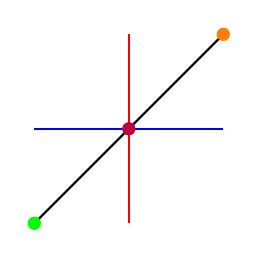
\begin{tikzpicture}[scale=1.2]
    \draw[thick] (0,0) -- (2,2);
    \draw[red, thick] (1,0) -- (1,2);
    \draw[blue, thick] (0,1) -- (2,1);
    \fill[green] (0,0) circle (2pt);
    \fill[orange] (2,2) circle (2pt);
    \fill[purple] (1,1) circle (2pt);
\end{tikzpicture}
\end{center}

\footnotesize
\texttt{\textbackslash draw[thick] (0,0) -- (2,2);}\\
\texttt{\textbackslash fill[green] (0,0) circle (2pt);}
\end{frame}